\section{Introdução}

\begin{frame}[fragile]{Unicórnio das linguagens}
\begin{figure}[ht!]
  \centering
  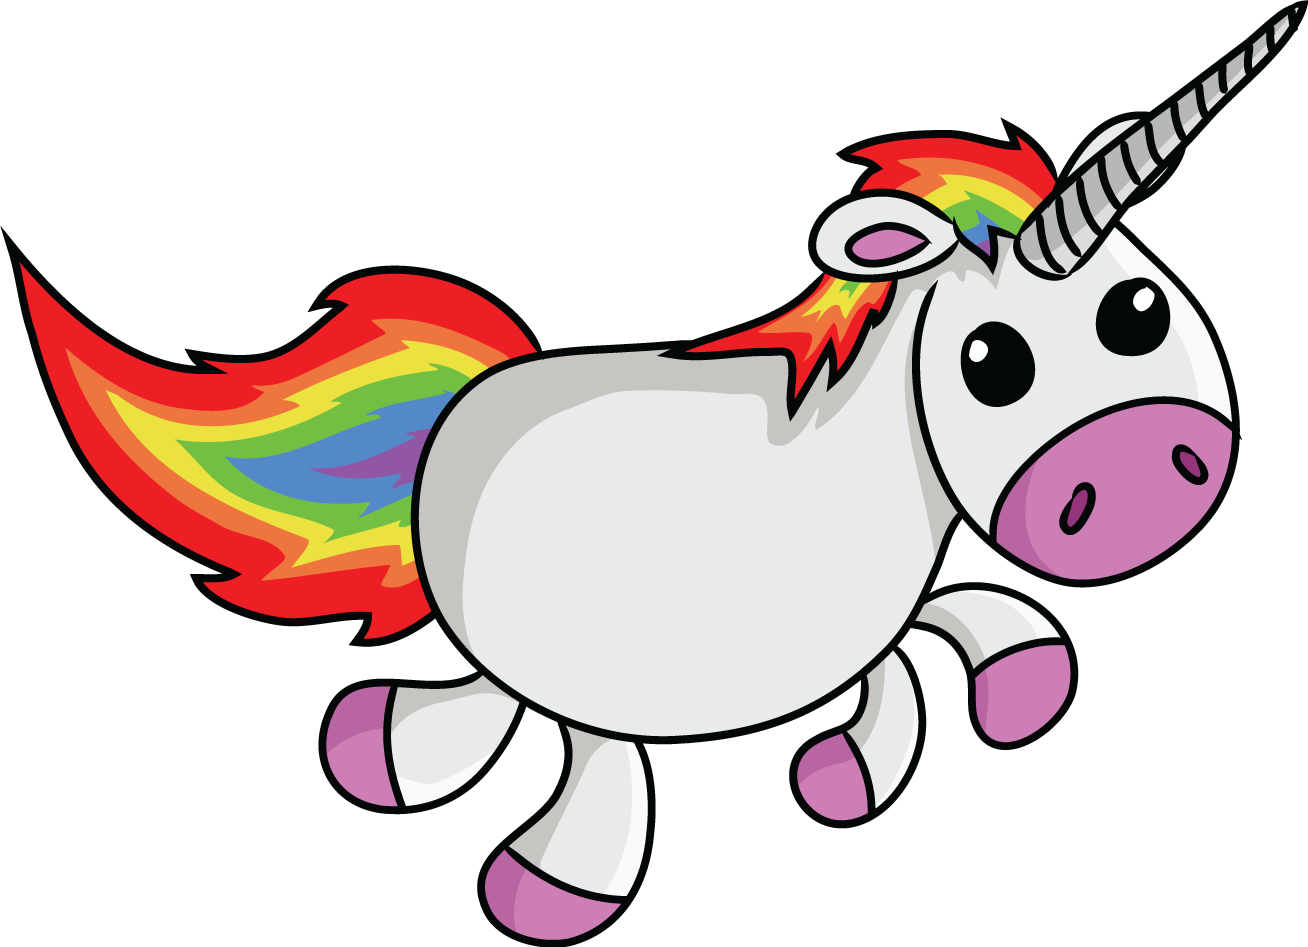
\includegraphics[scale=0.19]{images/unicorn.png}
\end{figure}
\begin{center}
\small{Linguagem orientada a unicórnios!}
\end{center}

\begin{center}
\small{Sem referências a linguagem \cancel{Unicon}
https://pt.wikipedia.org/wiki/Unicon}
\end{center}
\end{frame}

\begin{frame}[fragile]{HOPL (A history of the history of programming languages)}
\begin{figure}[ht!]
  \centering
  \includegraphics[width=\linewidth, height=6cm]{images/hopl.pdf}
\end{figure}

\begin{center}
\small{Estima-se que desde da década de 50 mais de 8.945 linguagens de programação foram criadas, uma média de 130 novas linguagens por ano.}
\end{center}

\begin{center}
Pouco mais de \textbf{1\%} das novas linguagens são consideradas \textbf{hype}.
\end{center}
\end{frame}